% Diagram: Parasitology and Cybersecurity - A Systems Perspective
% This diagram visually represents the parallels between biological parasites and cybersecurity threats
% Created for the manuscript "Parasites and Hackers: Vulnerabilities, Adaptations, and Systemic Insights"

\documentclass{article}
\usepackage{tikz}
\usepackage{adjustbox}
\begin{document}

\begin{figure}[h]
    \centering
    \adjustbox{scale=1.2,center}{
    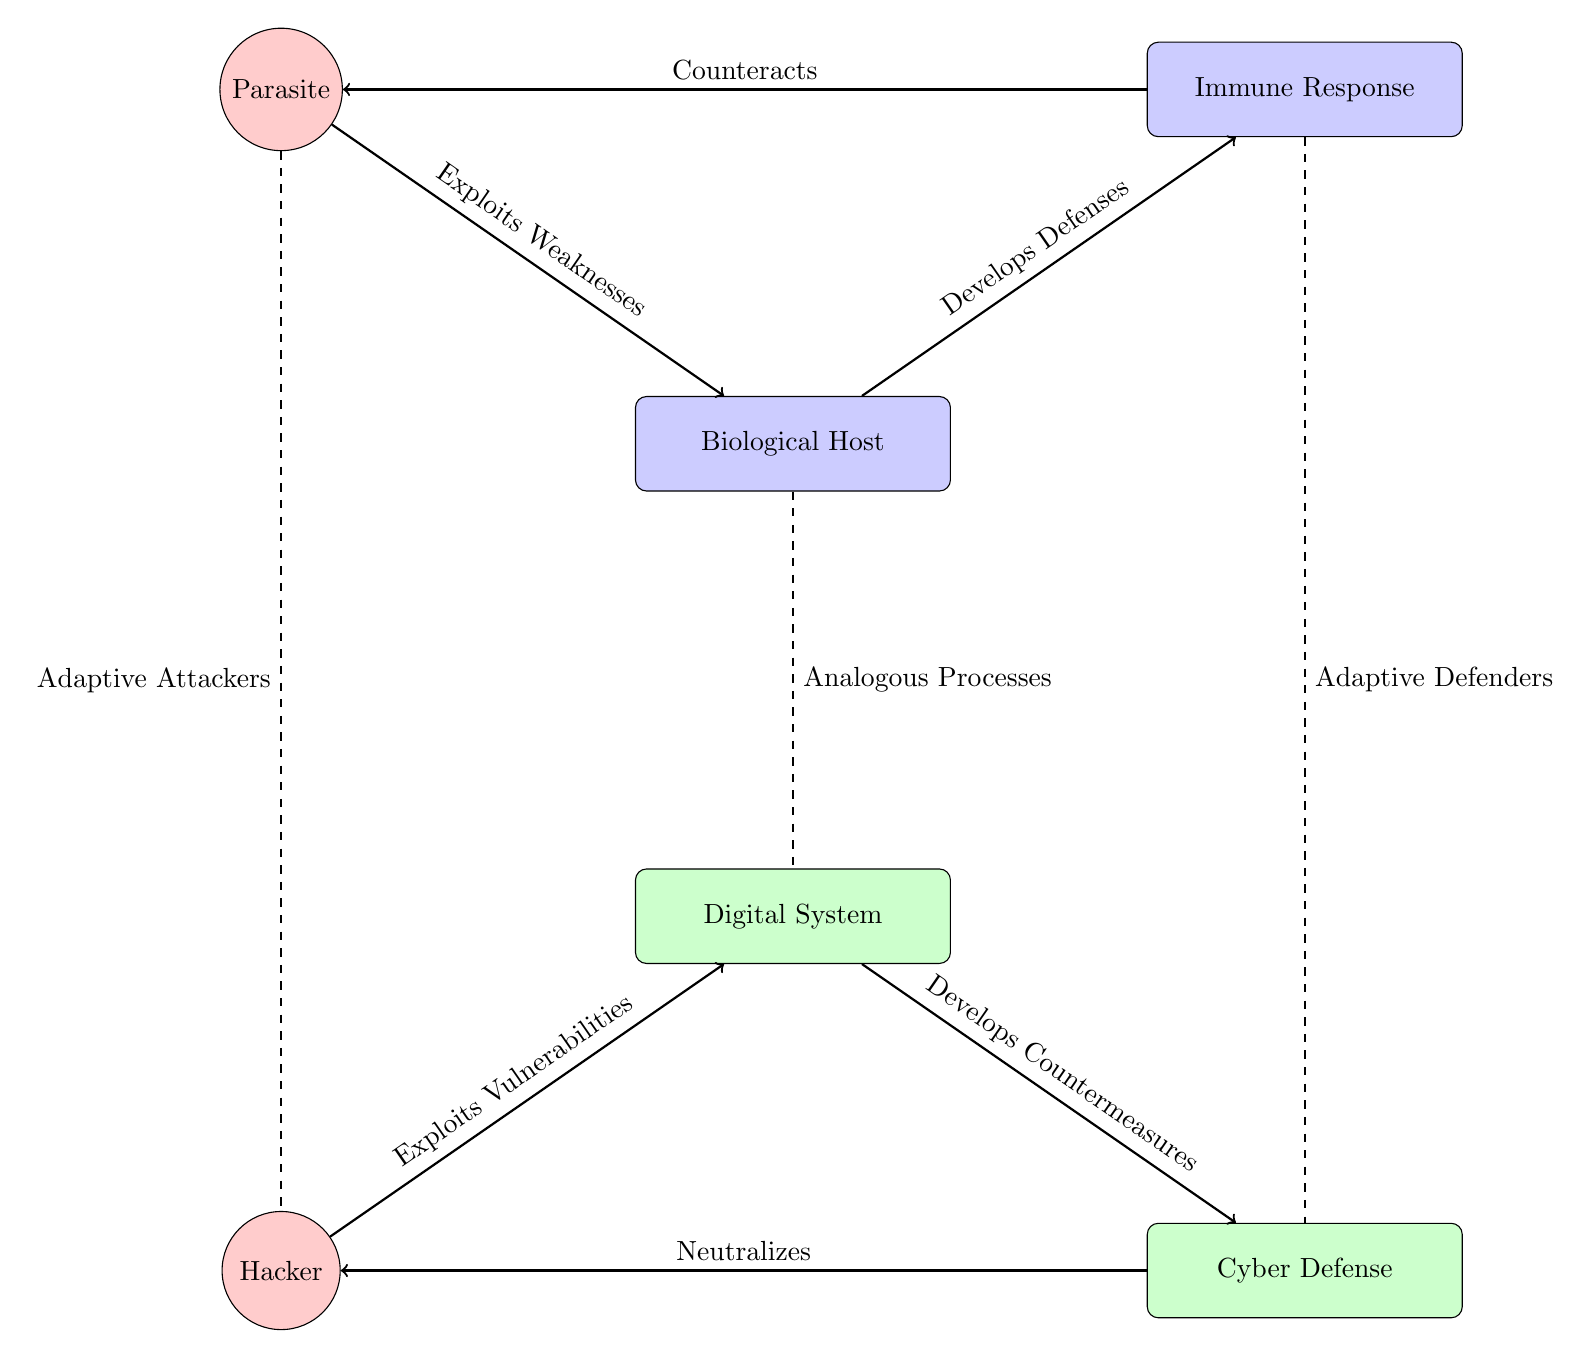
\begin{tikzpicture}
        % Biological System
        \node[draw, rectangle, rounded corners, fill=blue!20, minimum width=4cm, minimum height=1.2cm] (host) at (0,3) {Biological Host};
        \node[draw, circle, fill=red!20, minimum size=1.5cm] (parasite) at (-6.5,7.5) {Parasite};
        \node[draw, rectangle, rounded corners, fill=blue!20, minimum width=4cm, minimum height=1.2cm] (immune) at (6.5,7.5) {Immune Response};
        
        \draw[->, thick] (parasite) -- (host) node[midway, above, sloped] {Exploits Weaknesses};
        \draw[->, thick] (host) -- (immune) node[midway, above, sloped] {Develops Defenses};
        \draw[->, thick] (immune) -- (parasite) node[midway, above, sloped] {Counteracts};
        
        % Cybersecurity System
        \node[draw, rectangle, rounded corners, fill=green!20, minimum width=4cm, minimum height=1.2cm] (network) at (0,-3) {Digital System};
        \node[draw, circle, fill=red!20, minimum size=1.5cm] (hacker) at (-6.5,-7.5) {Hacker};
        \node[draw, rectangle, rounded corners, fill=green!20, minimum width=4cm, minimum height=1.2cm] (security) at (6.5,-7.5) {Cyber Defense};
        
        \draw[->, thick] (hacker) -- (network) node[midway, above, sloped] {Exploits Vulnerabilities};
        \draw[->, thick] (network) -- (security) node[midway, above, sloped] {Develops Countermeasures};
        \draw[->, thick] (security) -- (hacker) node[midway, above, sloped] {Neutralizes};
        
        % Parallels between systems
        \draw[dashed, thick] (host) -- (network) node[midway, right] {Analogous Processes};
        \draw[dashed, thick] (parasite) -- (hacker) node[midway, left] {Adaptive Attackers};
        \draw[dashed, thick] (immune) -- (security) node[midway, right] {Adaptive Defenders};
    \end{tikzpicture}}
    \caption{A Comparative Model of Biological and Cybersecurity Threat Adaptation}
    \label{fig:adaptation_model}
\end{figure}

\end{document}